\chapter{Validación modelo (3.2)}

Se presenta a continuación la validación del modelo (3.2) que se aplicó a los 3 sorteos. Se observa que para todos los sorteos el modelo ajustado cumple con los supuestos de una regresión lineal múltiple. En las gráficas \textbf{\textit{Residuals vs Fitted}} no se observa alguna tendencia y los puntos se ven aleatorios, de esta forma no observamos la existencia de problemas de heterocedasticidad. En las gráficas \textbf{\textit{Normal Q-Q}} observamos que los cuantiles de los residuales están alineados con los cuantiles teóricos de una distribución normal. Por otro lado, en ningún modelo se encontraron datos influyentes o atípicos.

\begin{figure}[H]
\centering
\label{fig:Validacion_mod2}
\begin{subfigure}
  \centering
  \caption{Validación modelo (3.2) AventuraT}
  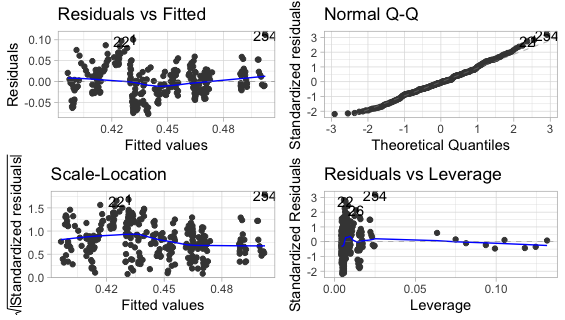
\includegraphics[width=.85\linewidth]{Imagenes/cuadritco_aven.png}
\end{subfigure}%
\begin{subfigure}
  \centering
  \caption{Validación modelo (3.2) Educativo}
  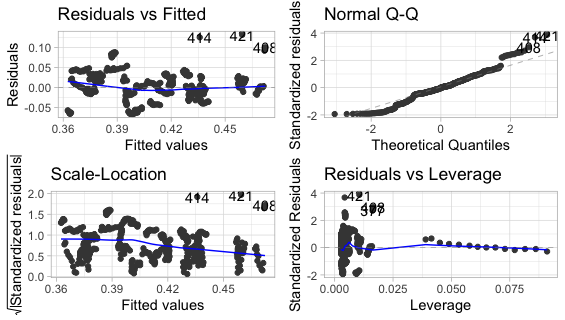
\includegraphics[width=.85\linewidth]{Imagenes/cuadratico_educ.png}
\end{subfigure}
\end{figure}

\begin{figure}[H]
\centering
\label{fig:Validacion_modelo2}
\begin{subfigure}
  \centering
  \caption{Validación modelo (3.2) Mi Sueño}
  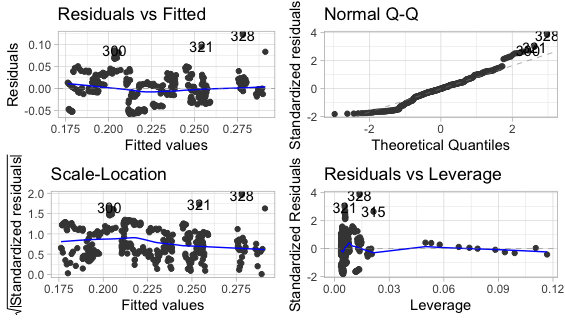
\includegraphics[width=.85\linewidth]{Imagenes/cuadratico_suen.png}
\end{subfigure}%
\end{figure}

De igual forma, se aplicó la prueba Jarque-Bera para probar la normalidad en los residuales. Se obtivieron los siguientes resultados:

%------Tabla

\begin{table}[H]
\centering
\begin{tabular}{@{}lrrlr@{}}
\toprule
\multicolumn{5}{c}{Jarque-Bera Test}                                                                \\ \midrule
\multicolumn{1}{c}{Sorteo} & \multicolumn{1}{c}{} & \multicolumn{1}{c}{Estadístico JB} &  & p-value \\ \midrule
AventuraT                  &                      & 0.35167                            &  & 0.821  \\
Educativo                  &                      & 2.2201                             &  & 0.2685   \\
Mi Sueño                   &                      & 3.4852                             &  & 0.1315   \\ \bottomrule
\end{tabular}
\end{table}

%---------

De esta forma, observamos que los modelos son válidos y justifican estadísticamente la utilización de los coeficientes estimados por el modelo (3.2) utilizados en esta tesis.